\chapter{Results}
\label{ch:result}

	\section{Forest definition and accuracy assessment}
	\label{sec:forest_definition}
	%TODO samples and jaccard scores as csv to github
	%TODO jaccard change order to americas, asia, africa

		\begin{figure}[ht]
			\centering
			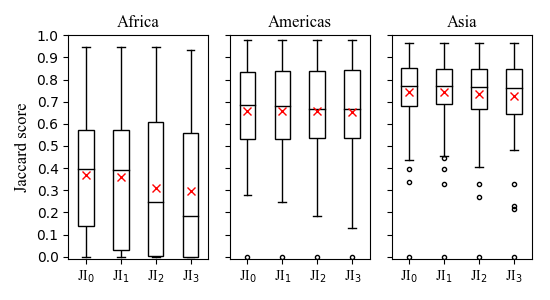
\includegraphics[scale=1]{img/jaccard}
			\caption[Similarity distribution of \ac{GFC} tree cover vs. \ac{GL30} tree cover at 200]{\textbf{Similarity distribution of \ac{GFC} tree cover vs. \ac{GL30} tree cover at 2000:} Americas from JC$_0$ till JC$_3$: $\bar{x}\approxeq$ .71, .71, .70, .69; $\tilde{x}\approxeq$ .77, .77, .76, .75; $Q_1\approxeq$ .64, .65, .64, .63; $Q_3\approxeq$ .84, .84, .84, .83; Asia from JC$_0$ till JC$_3$: $\bar{x}\approxeq$ .71, .71, .70, .69; $\tilde{x}\approxeq$ .77, .77, .76, .75; $Q_1\approxeq$ .65, .66, .64, .63; $Q_3\approxeq$ .84, .84, .84, .83; Africa from JC$_0$ till JC$_3$: $\bar{x}\approxeq$ .39, .39, .34, .32; $\tilde{x}\approxeq$ .40, .40, .31, .29; $Q_1\approxeq$ .14, .10, .00, .00; $Q_3\approxeq$ .60, .61, .63, .56}
			\label{fig:jaccard}
		\end{figure}

		\begin{table}[ht]
			\centering
			\caption[Two-sided Wilcoxon signed-rank test]{\textbf{Two-sided Wilcoxon signed-rank test:}}
			\label{tab:wilcoxontwosided}
			\begin{tabular}{lrrrrrrrrrrrr}
				\hline
				& \multicolumn{12}{c}{H$_0$: $\tilde{x_1}=\tilde{x_2}$} \\\hline
				& \multicolumn{4}{c}{Americas} & \multicolumn{4}{c}{Asia} & \multicolumn{4}{c}{Africa} \\
				Cls & JI$_0$ & JI$_1$ & JI$_2$ & JI$_3$ & JI$_0$ & JI$_1$ & JI$_2$ & JI$_3$ & JI$_0$ & JI$_1$ & JI$_2$ & JI$_3$ \\\hline
				JI$_0$ & 1. &  &  &  & 1. &  &  &  & 1. &  &  & \\
				JI$_1$ & .00 & 1. &  &  & .72 & 1. &  &  & .22 & 1. &  & \\
				JI$_2$ & .06 & .36 & 1. &  & .00 & .00 & 1. &  & .03 & .03 & 1. & \\
				JI$_3$ & .16 & .50 & .60 & 1. & .00 & .00 & .00 & 1. & .00 & .00 & .00 & 1. \\\hline
			\end{tabular}
		\end{table}

		\begin{table}[ht]
			\centering
			\caption[One-sided Wilcoxon signed-rank test]{\textbf{One-sided Wilcoxon signed-rank test:}}
			\label{tab:wilcoxononesided}
			\begin{tabular}{llrrrrrrrrrrrr}
				\hline
				& & \multicolumn{12}{c}{H$_0$: $\tilde{x_1}\leq\tilde{x_2}$} \\\hline
				& & \multicolumn{4}{c}{Americas} & \multicolumn{4}{c}{Asia} & \multicolumn{4}{c}{Africa} \\
				& Cls & JI$_0$ & JI$_1$ & JI$_2$ & JI$_3$ & JI$_0$ & JI$_1$ & JI$_2$ & JI$_3$ & JI$_0$ & JI$_1$ & JI$_2$ & JI$_3$ \\\hline
				\multirow{4}{*}{\STAB{\rotatebox[origin=c]{90}{H$_0$: $\tilde{x_1}\geq\tilde{x_2}$}}} & JI$_0$ & 1. & .00 & .03 & .08 & 1. & .64 & 1. & 1. & 1. & .11 & .98 & 1. \\
				& JI$_1$ & 1. & 1. & .18 & .25 & .36 & 1. & 1. & 1. & .89 & 1. & .99 & 1. \\
				& JI$_2$ & .97 & .82 & 1. & .30 & .00 & .00 & 1. & 1. & .02 & .01 & 1. & 1. \\
				& JI$_3$ & .92 & .75 & .70 & 1. & .00 & .00 & .00 & 1. & .00 & .00 & .00 & 1. \\\hline
			\end{tabular}
		\end{table}

		\begin{table}[ht]
			\centering
			\caption[Accuracy assessment]{Confusion matrix for accuracy assessment}
			\label{tab:accuracy}
			\begin{tabular}{llrrrrrrrrrrrr}
				\hline
				& & \multicolumn{9}{c}{Reference} & & & \\
				& Cls & 10 & 20 & 25 & 30 & 40 & 50 & 60 & 80 & 90 & Tot & UAc & Om \\\hline
				\multirow{9}{*}{\STAB{\rotatebox[origin=c]{90}{Prediction}}}
				& 10 & 732 & 38 & 62 & 15 & 16 & 2 & 3 & 5 & 0 & 873 & .84 & .16 \\ 
				& 20 & 42 & 751 & 57 & 189 & 31 & 12 & 0 & 17 & 4 & 1103 & .68 & .32 \\ 
				& 25 & 29 & 202 & 1155 & 173 & 22 & 10 & 5 & 11 & 4 & 1611 & .72 & .28 \\ 
				& 30 & 36 & 187 & 32 & 1466 & 73 & 21 & 0 & 17 & 0 & 1832 & .80 & .20 \\ 
				& 40 & 14 & 21 & 4 & 41 & 352 & 1 & 1 & 2 & 1 & 437 & .81 & .19 \\ 
				& 50 & 0 & 5 & 3 & 10 & 4 & 50 & 0 & 1 & 0 & 73 & .68 & .32 \\ 
				& 60 & 2 & 1 & 0 & 3 & 0 & 2 & 18 & 2 & 0 & 28 & .64 & .36 \\ 
				& 80 & 3 & 4 & 0 & 1 & 1 & 1 & 0 & 50 & 0 & 60 & .83 & .17 \\ 
				& 90 & 0 & 0 & 0 & 1 & 0 & 0 & 0 & 3 & 5 & 9 & .56 & .44 \\\hline 
				& Tot & 858 & 1209 & 1313 & 1899 & 499 & 99 & 27 & 108 & 14 & 6026 & & \\
				& PAc & .85 & .62 & .88 & .77 & .71 & .51 & .67 & .46 & .36 & & \multicolumn{2}{r}{OvAc} \\
				& Com & .15 & .38 & .12 & .23 & .29 & .49 & .33 & .54 & .64 & & \multicolumn{2}{r}{.75} \\ \hline
			\end{tabular}
		\end{table}

\newpage

	\section{Deforestation drivers}
	\label{sec:driver}
	%TODO structure global followed by continental (americas, asia, africa is decreasing order)
	%TODO global bar-chart and continental
	%TODO add global column to table
	%TODO for top countries per continent estimates
	%TODO tree-cover and loss to one panel

		\subsection{Global}
			\begin{table}[ht]
				\centering
				\caption[Deforestation driver]{Absolute in km$^2$}
				\label{tab:driver_tab}
				\begin{tabular}{lcllrrr}
					Class & Code & Type & & Americas & Asia & Africa \\\hline
					\multirow{4}{*}{Agriculture} & \multirow{2}{*}{10} & \multirow{2}{*}{Cropland} & rel. & 24.37 & 18.37 & 25.01 \\
					& & & abs. & 95908 & 38719 & 44368 \\
					& \multirow{2}{*}{30} & \multirow{2}{*}{Grassland} & rel. & 46.19 & 8.41 & 50.46 \\
					& & & abs. & 181781 & 17726 & 89516 \\
					\multirow{4}{*}{Forestry/Plantations} & \multirow{2}{*}{25} & \multirow{2}{*}{Regrowth} & rel. & 14.40 & 70.27 & 18.61 \\
					& & & abs. & 56671 & 148111 & 33014 \\
					& \multirow{2}{*}{40} & \multirow{2}{*}{Shrubland} & rel. & 12.69 & 1.11 & 3.77 \\
					& & & abs. & 49941 & 2340 & 6688 \\
					\multirow{4}{*}{Urban/Mining} & \multirow{2}{*}{80} & \multirow{2}{*}{Artificial} & rel. & 0.41 & 0.46 & 0.71 \\
					& & & abs. & 1614 & 970 & 1260 \\
					& \multirow{2}{*}{90} & \multirow{2}{*}{Bareland} & rel. & 0.10 & 0.03 & 0.09 \\
					& & & abs. & 394 & 63 & 160 \\
					\multirow{4}{*}{Natural} & \multirow{2}{*}{50} & \multirow{2}{*}{Wetland} & rel. & 1.50 & 0.97 & 1.23 \\
					& & & abs. & 5903 & 2045 & 2182 \\
					& \multirow{2}{*}{60} & \multirow{2}{*}{Water} & rel. & 0.32 & 0.38 & 0.13 \\
					& & & abs. & 1259 & 801 & 231 \\\hline
					\multicolumn{3}{c}{\multirow{2}{*}{Forest loss}} & rel. & 3.87 & 4.68 & 1.69 \\
					& & & abs. & 393550 & 210774 & 177400 \\
					\multicolumn{3}{c}{Forest cover} & abs. & 10223187 & 4457940 & 10496591 \\\hline
				\end{tabular}
			\end{table}

		\subsection{Americas}
			\begin{figure}[ht]
				\centering
				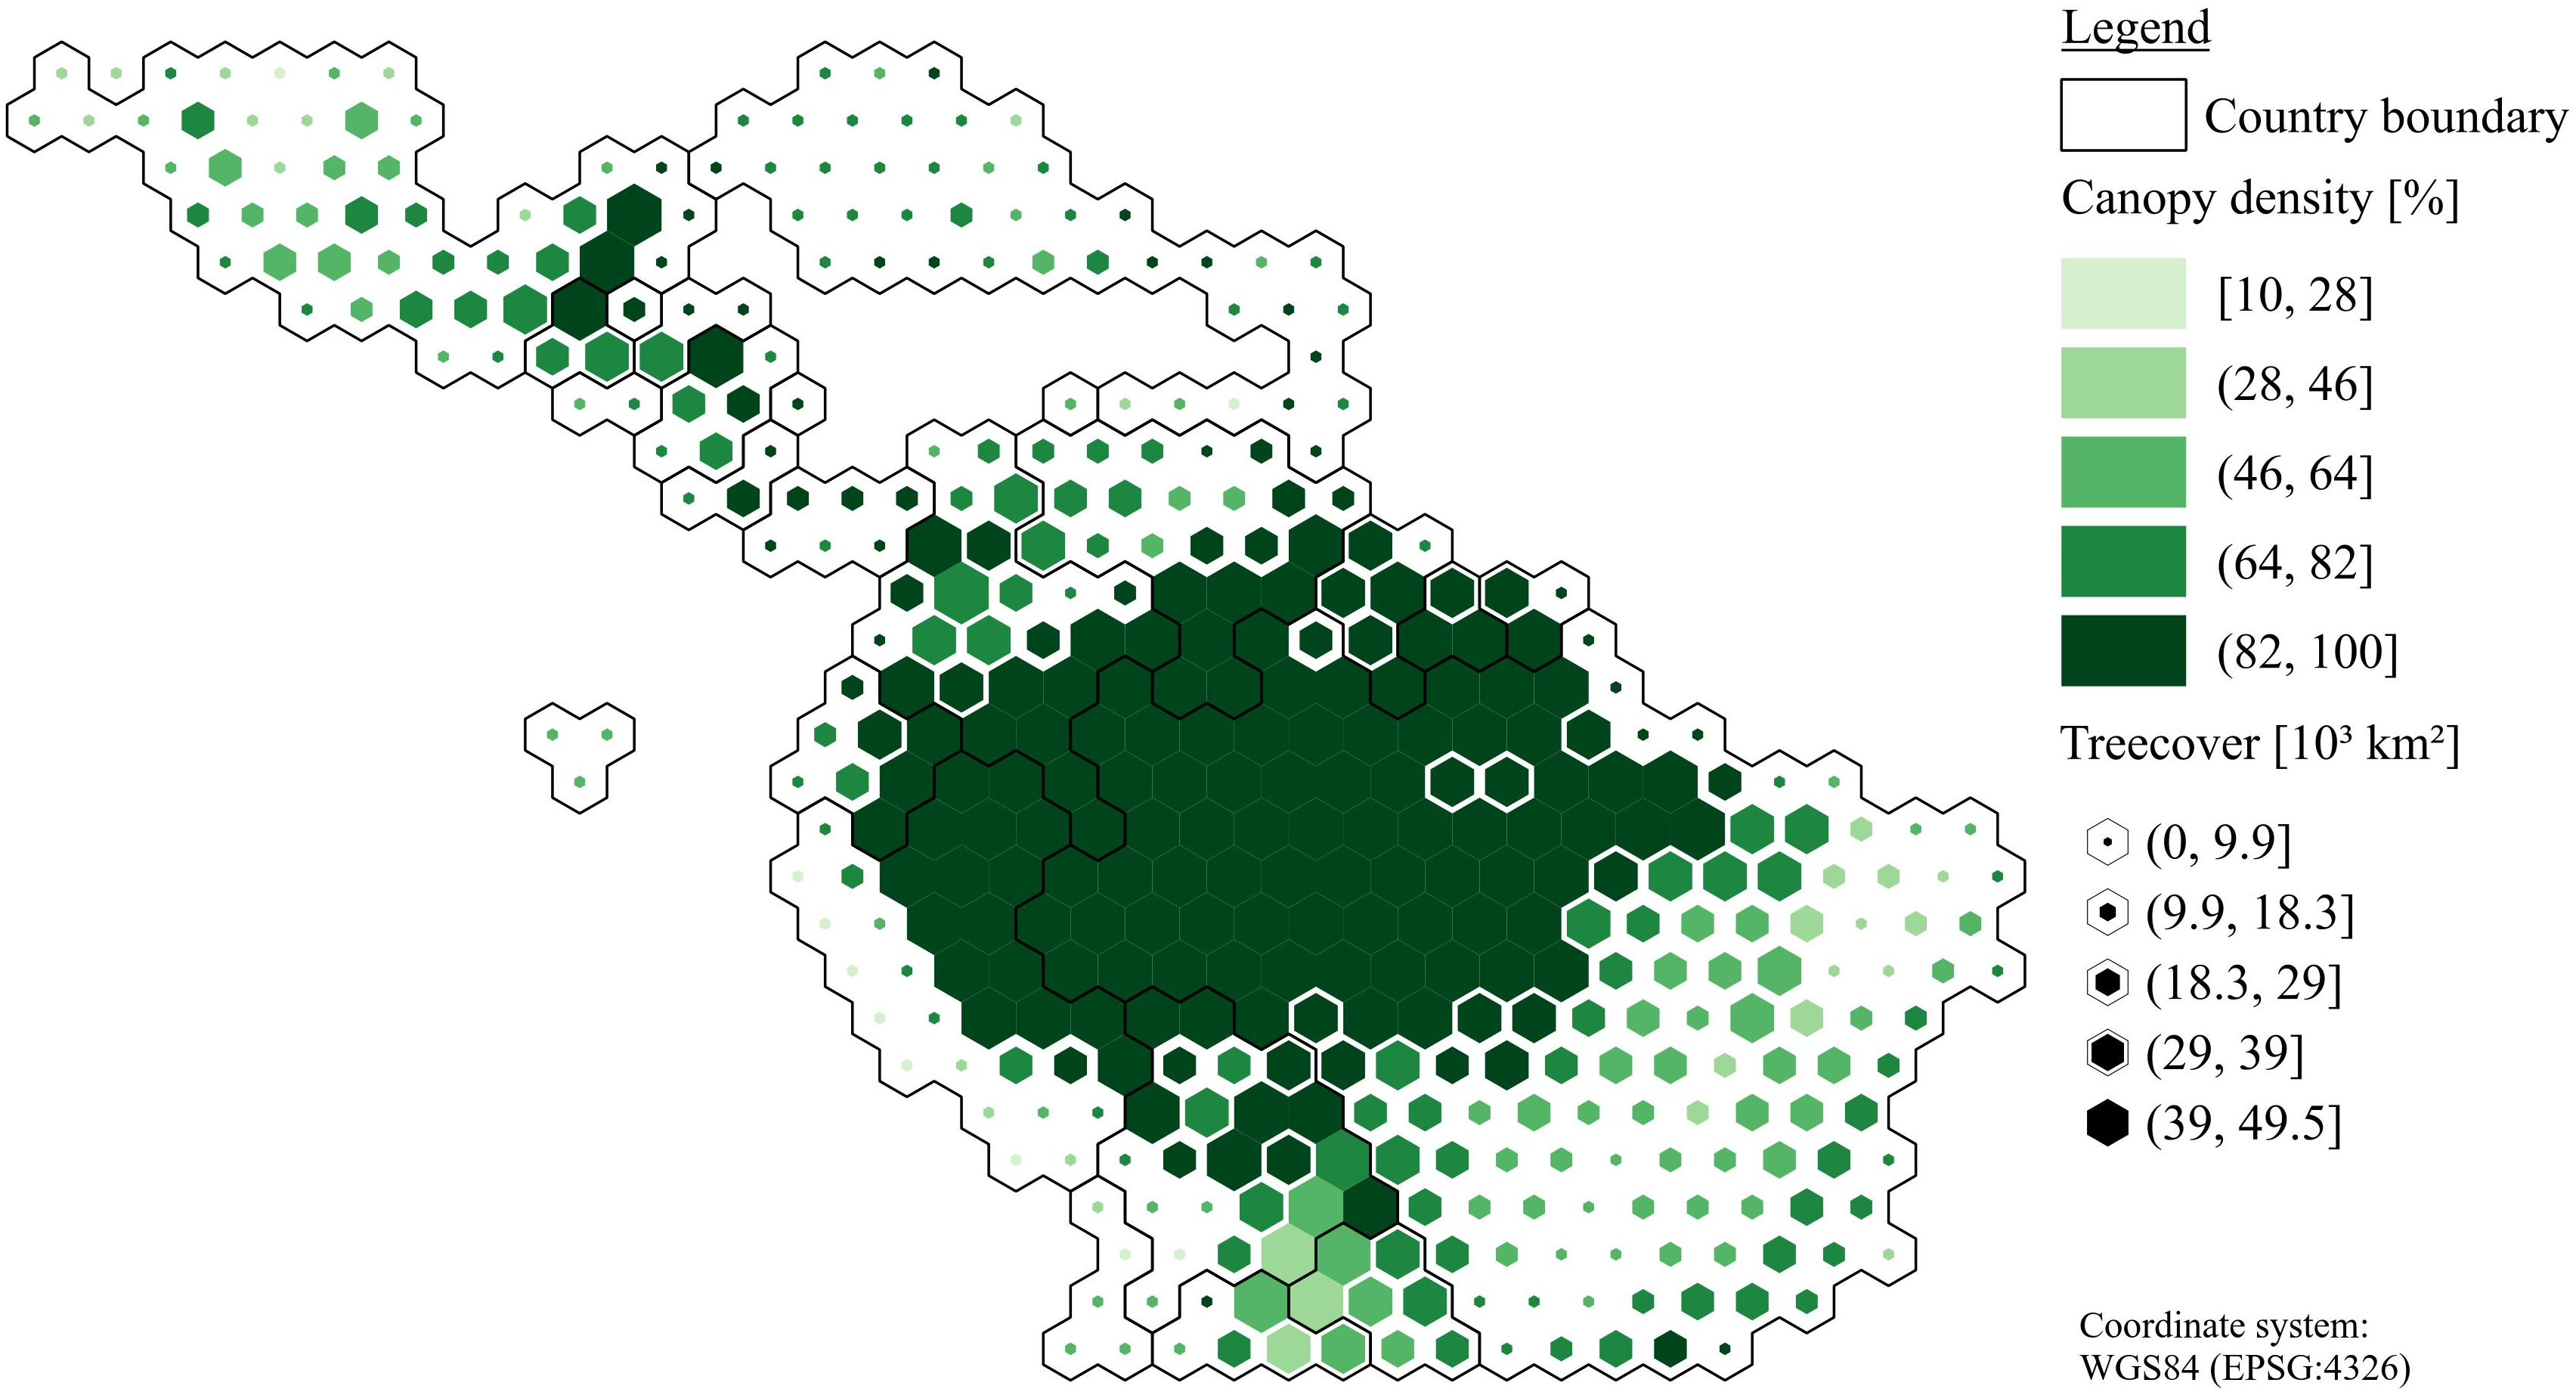
\includegraphics[scale=1]{img/americas_treecover_frameless}
				\caption[Ecosystem service values]{}
				\label{fig:americascover}
			\end{figure}
			\begin{figure}[ht]
				\centering
				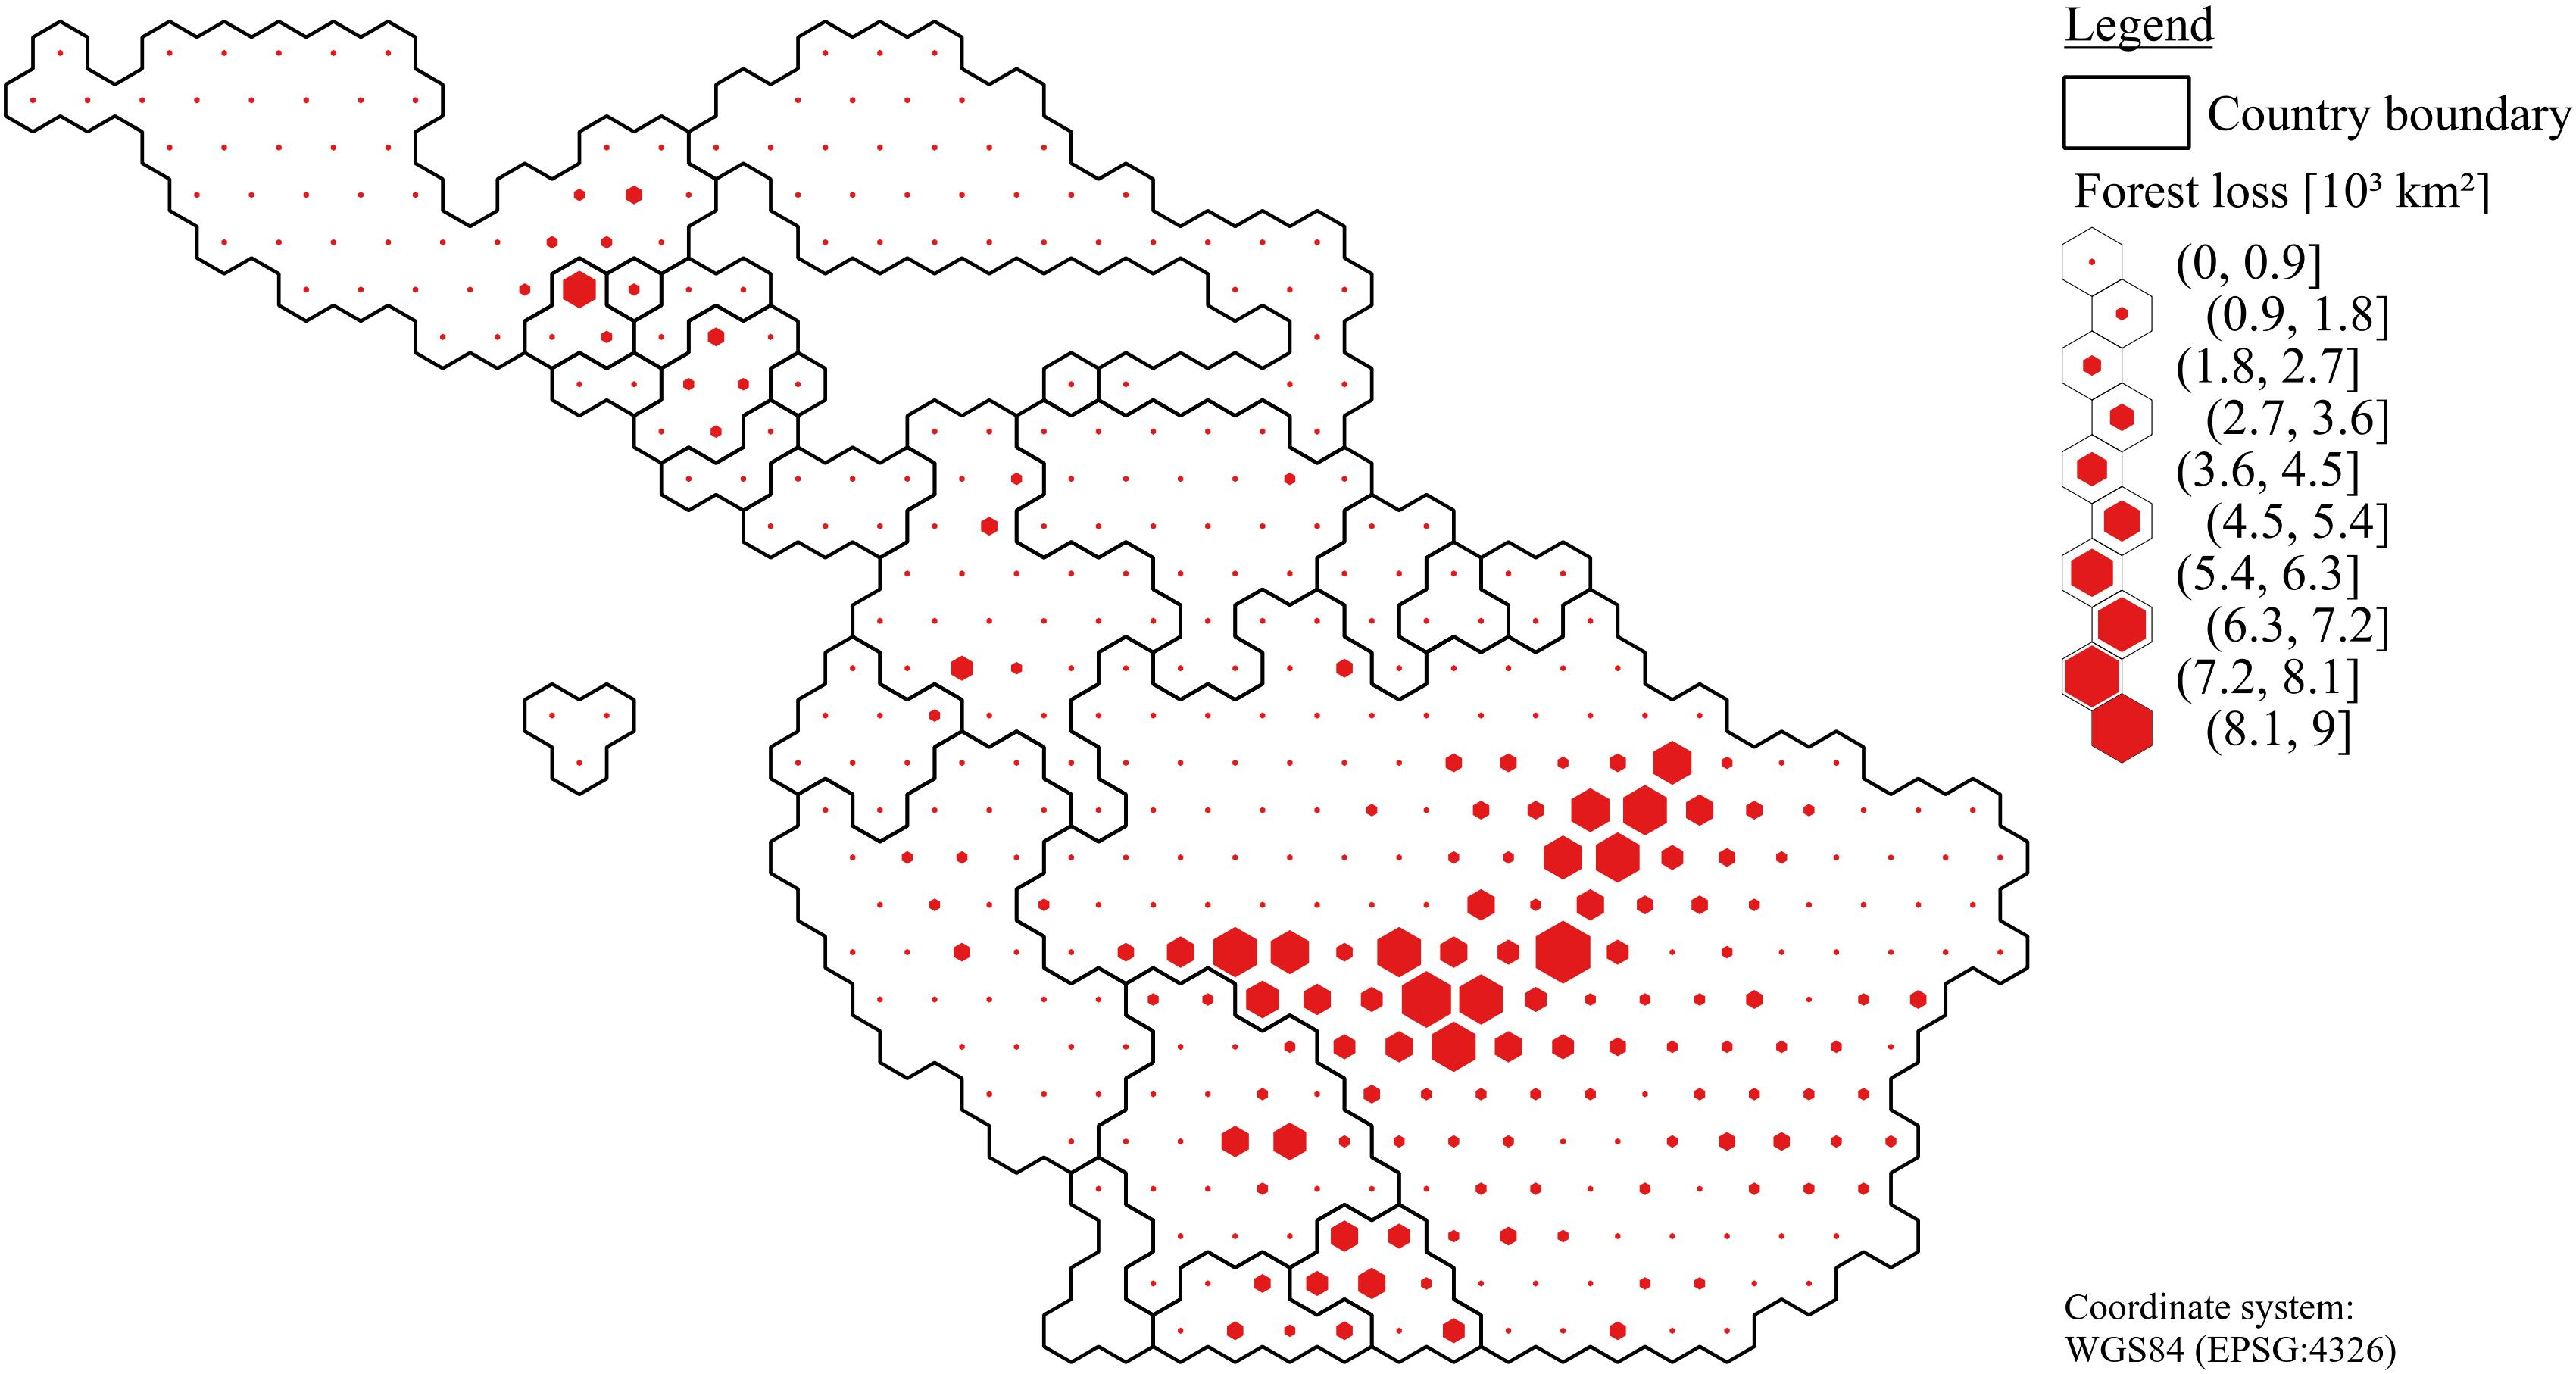
\includegraphics[scale=1]{img/americas_loss_frameless}
				\caption[Ecosystem service values]{}
				\label{fig:americasloss}
			\end{figure}
			\begin{figure}[ht]
				\centering
				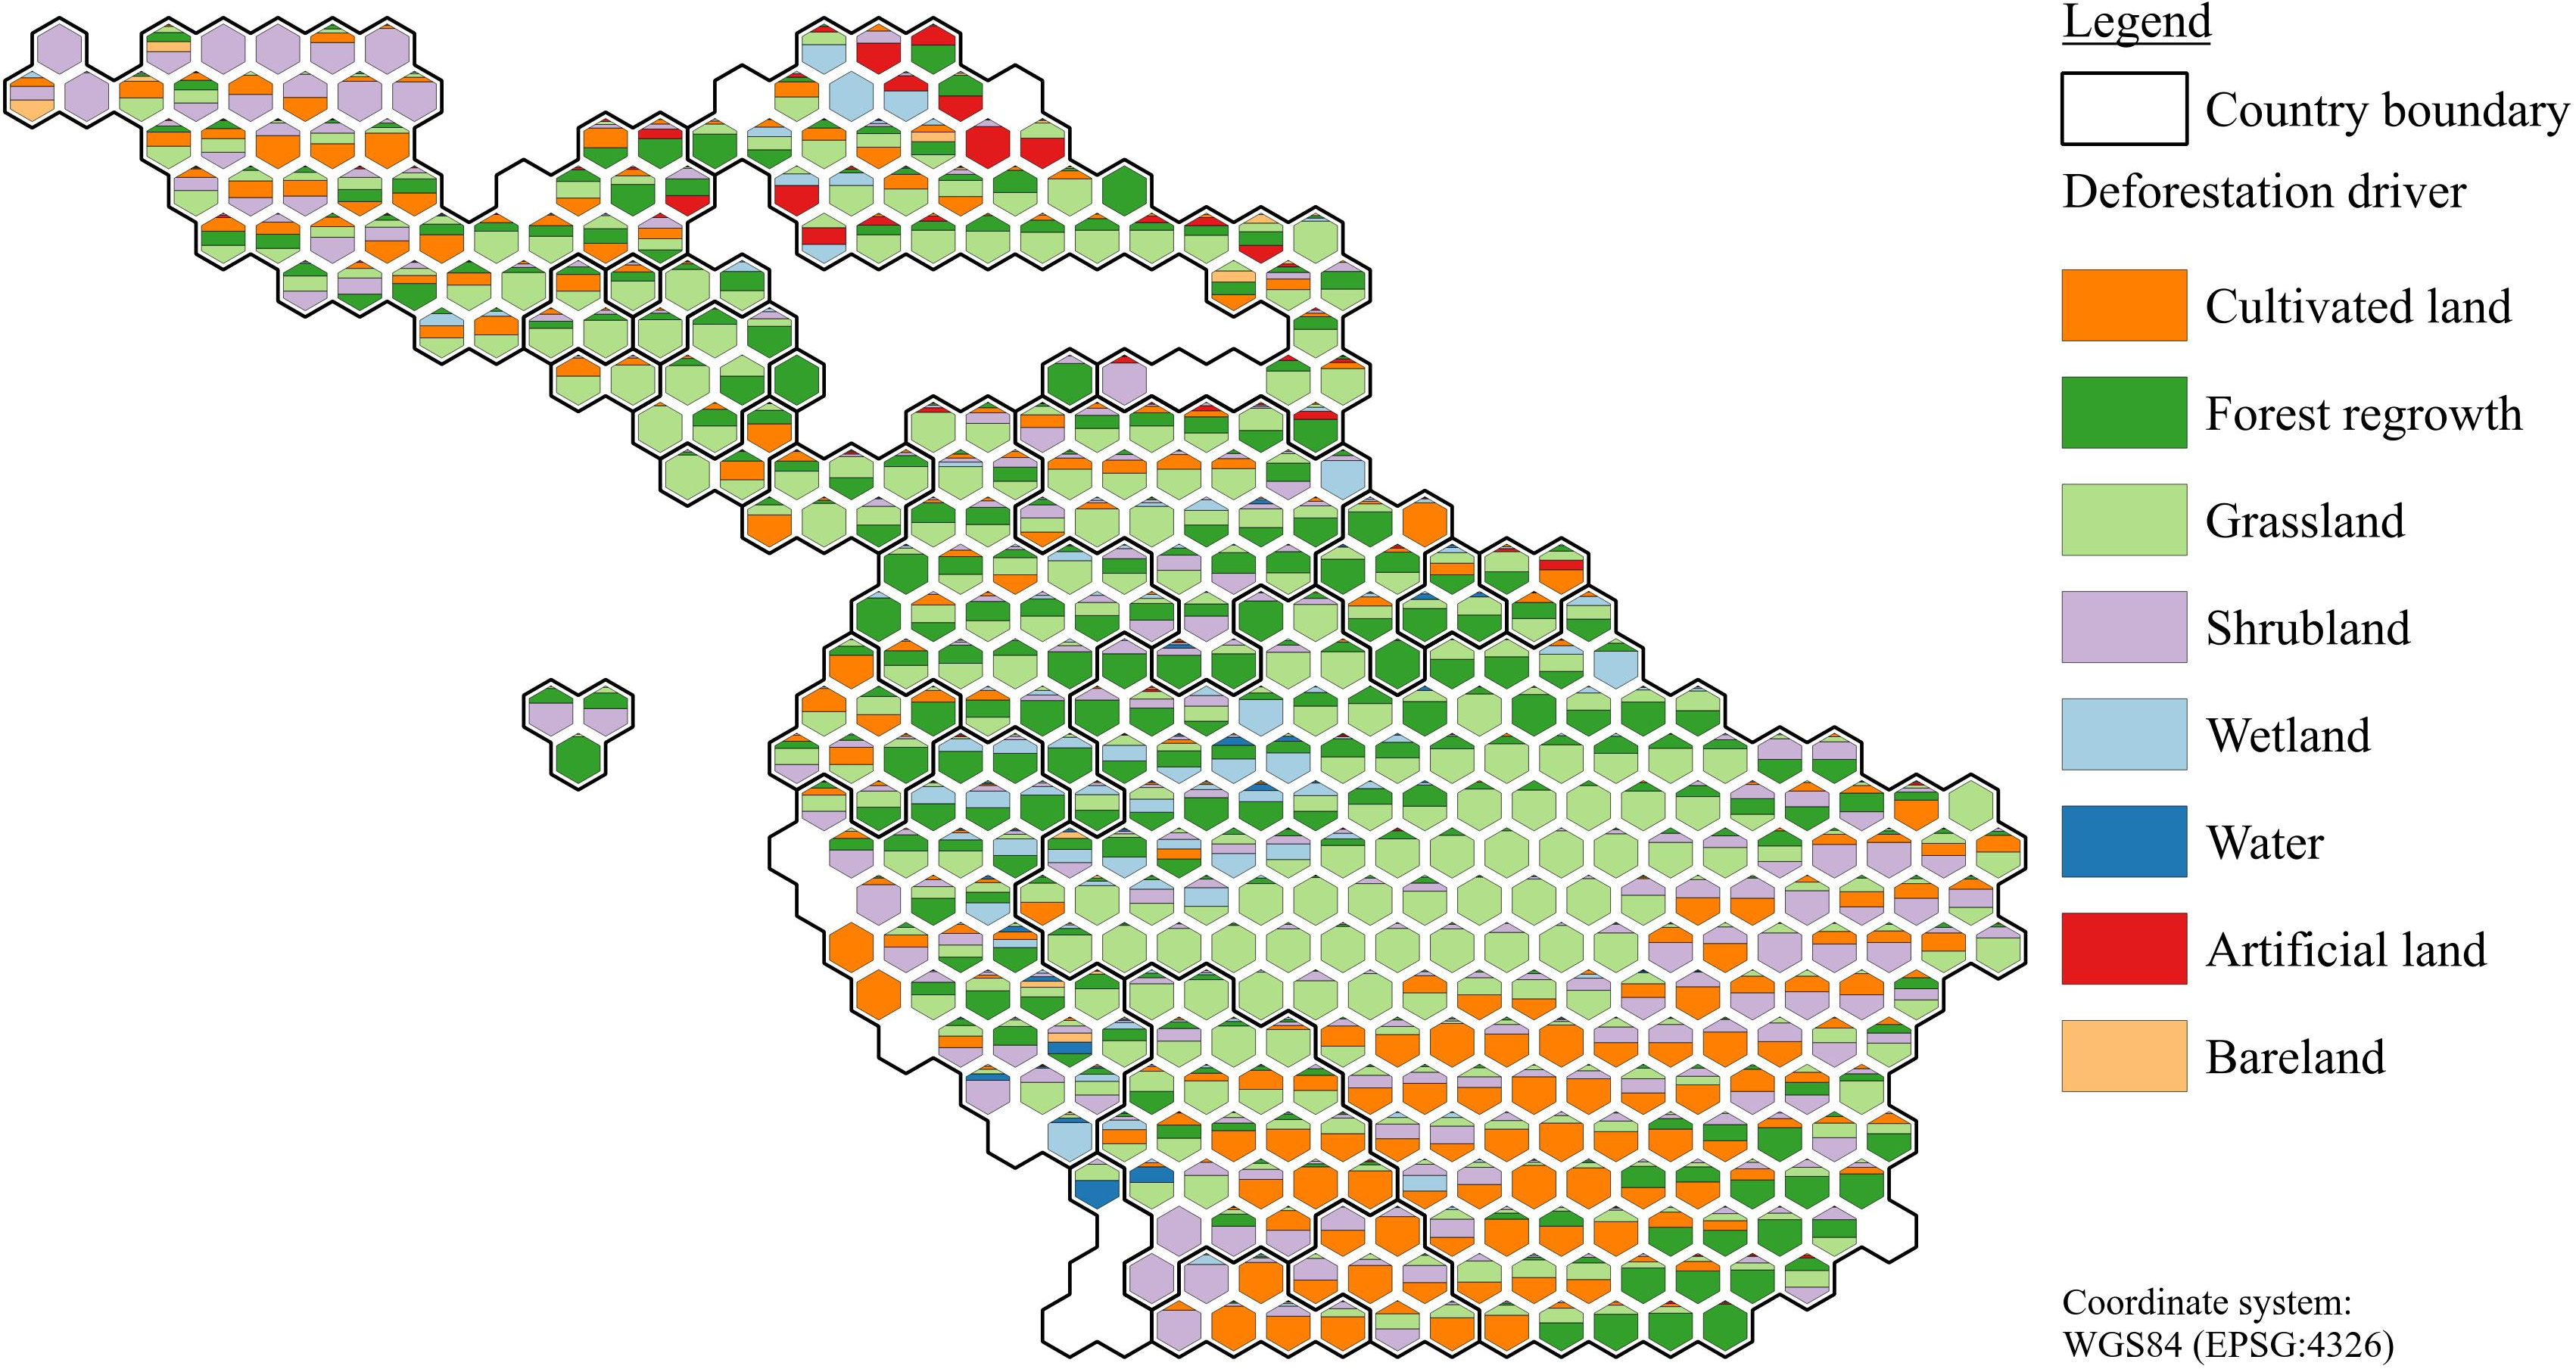
\includegraphics[scale=1]{img/americas_driver_frameless}
				\caption[Ecosystem service values]{}
				\label{fig:americasdriver}
			\end{figure}

		\subsection{Asia}
			\begin{figure}[ht]
				\centering
				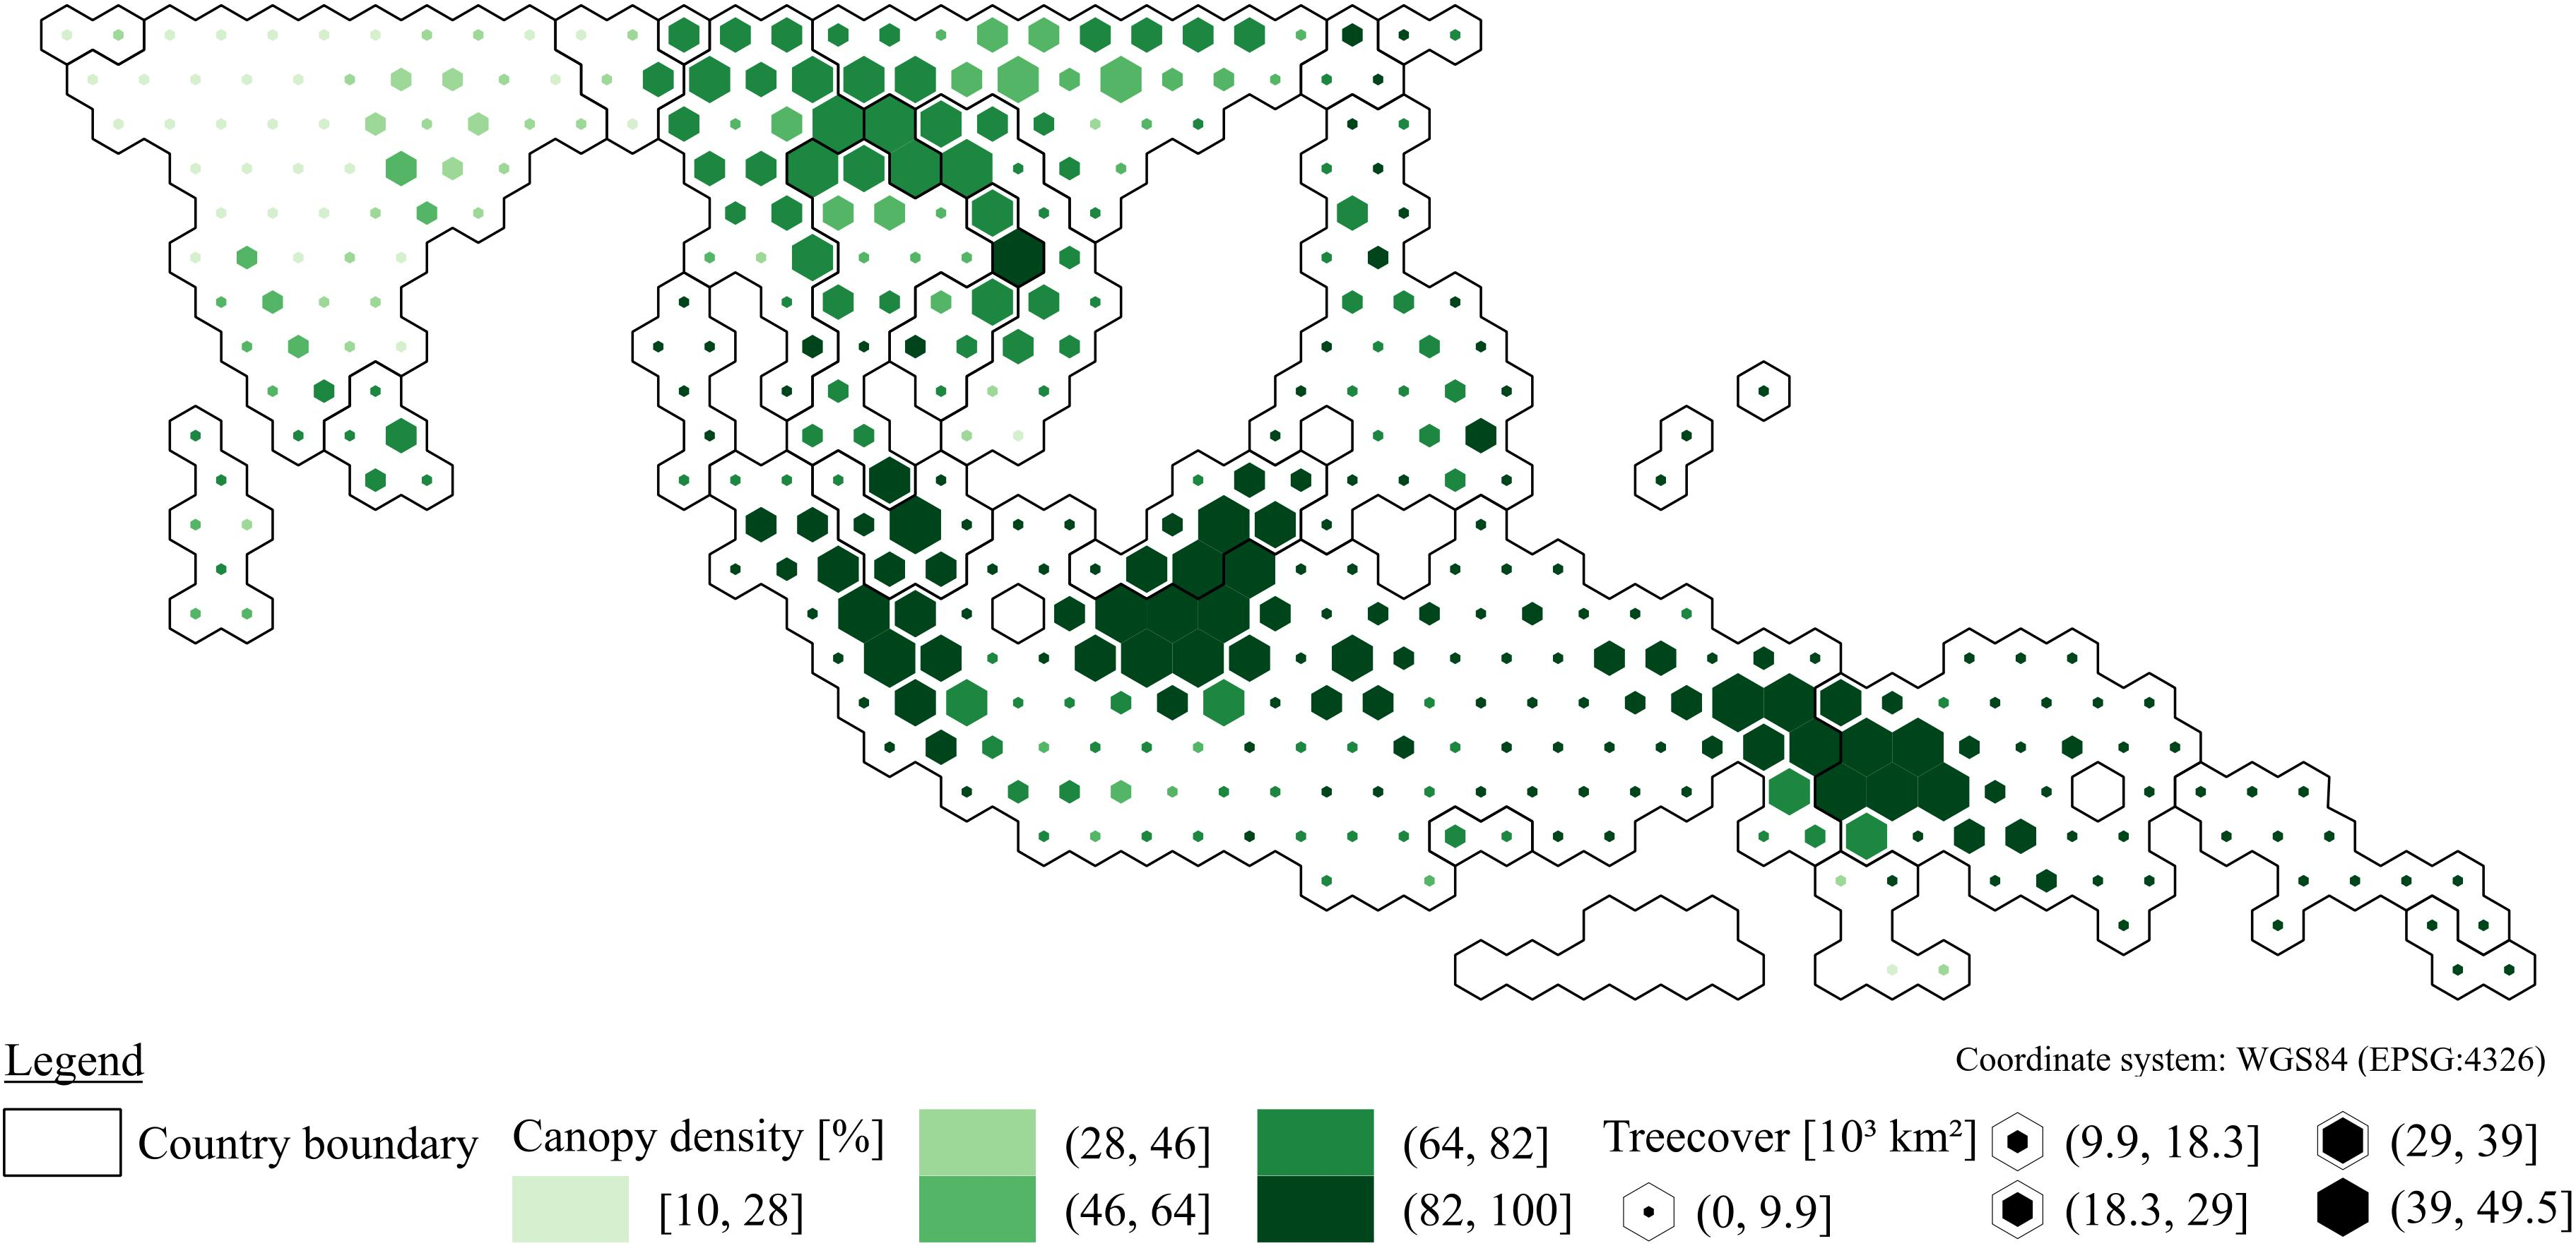
\includegraphics[scale=1]{img/asia_treecover_frameless}
				\caption[Ecosystem service values]{}
				\label{fig:asiacover}
			\end{figure}
			\begin{figure}[ht]
				\centering
				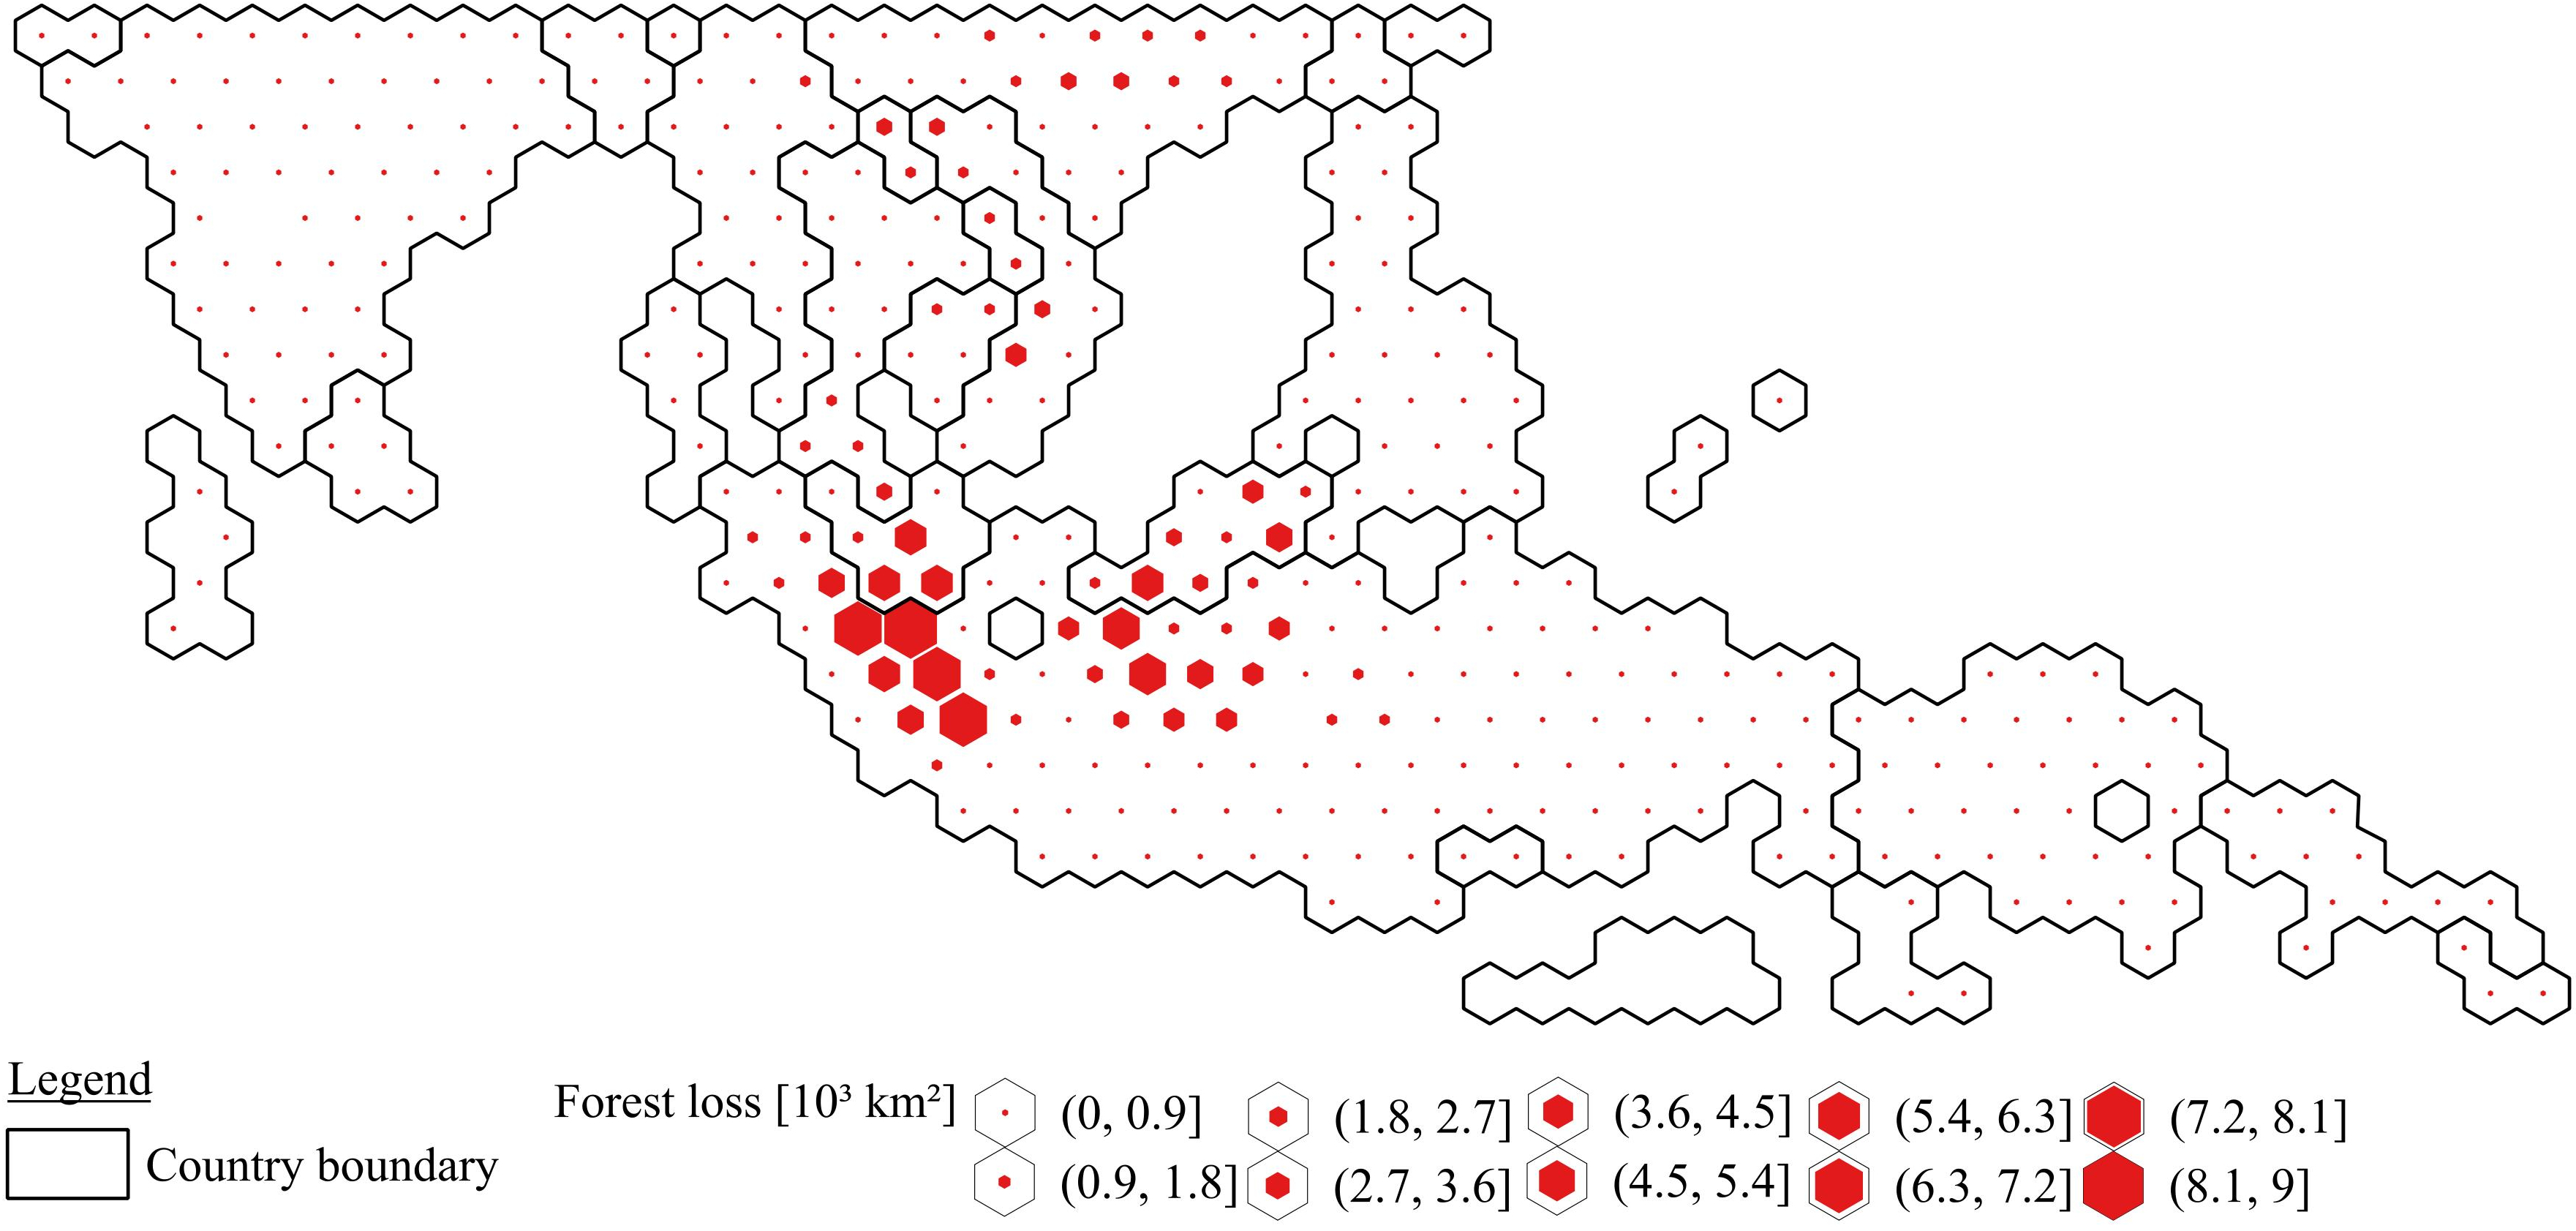
\includegraphics[scale=1]{img/asia_loss_frameless}
				\caption[Ecosystem service values]{}
				\label{fig:asialoss}
			\end{figure}
			\begin{figure}[ht]
				\centering
				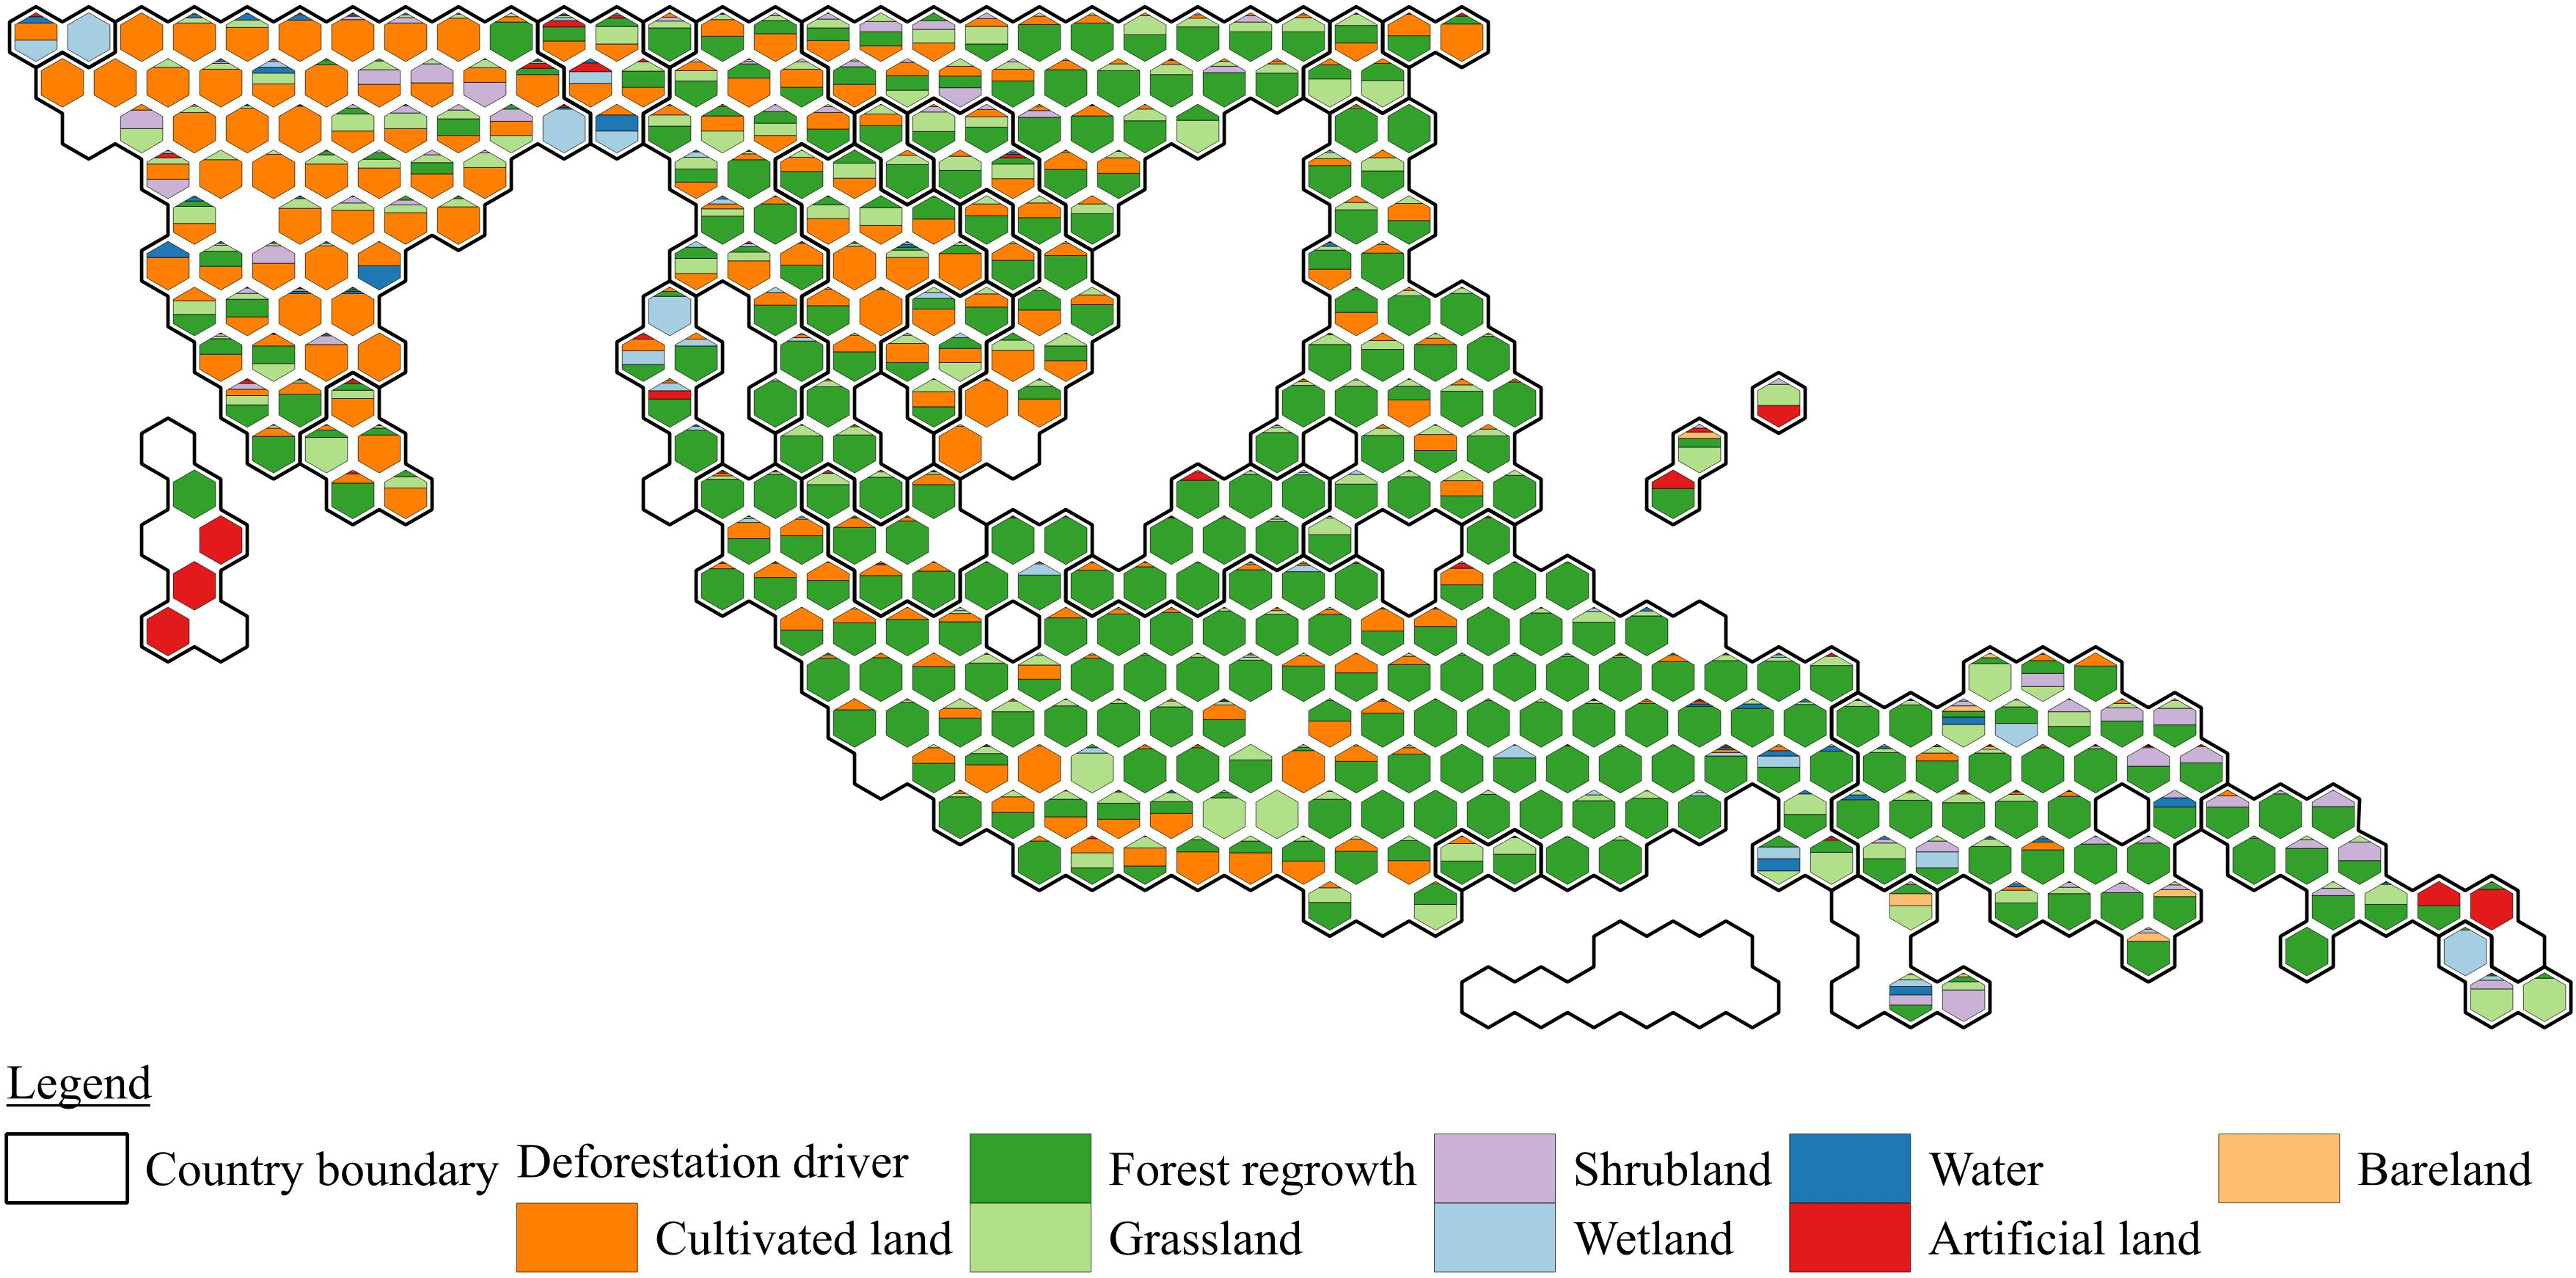
\includegraphics[scale=1]{img/asia_driver_frameless}
				\caption[Ecosystem service values]{}
				\label{fig:asiadriver}
			\end{figure}

		\subsection{Africa}
			\begin{figure}[ht]
				\centering
				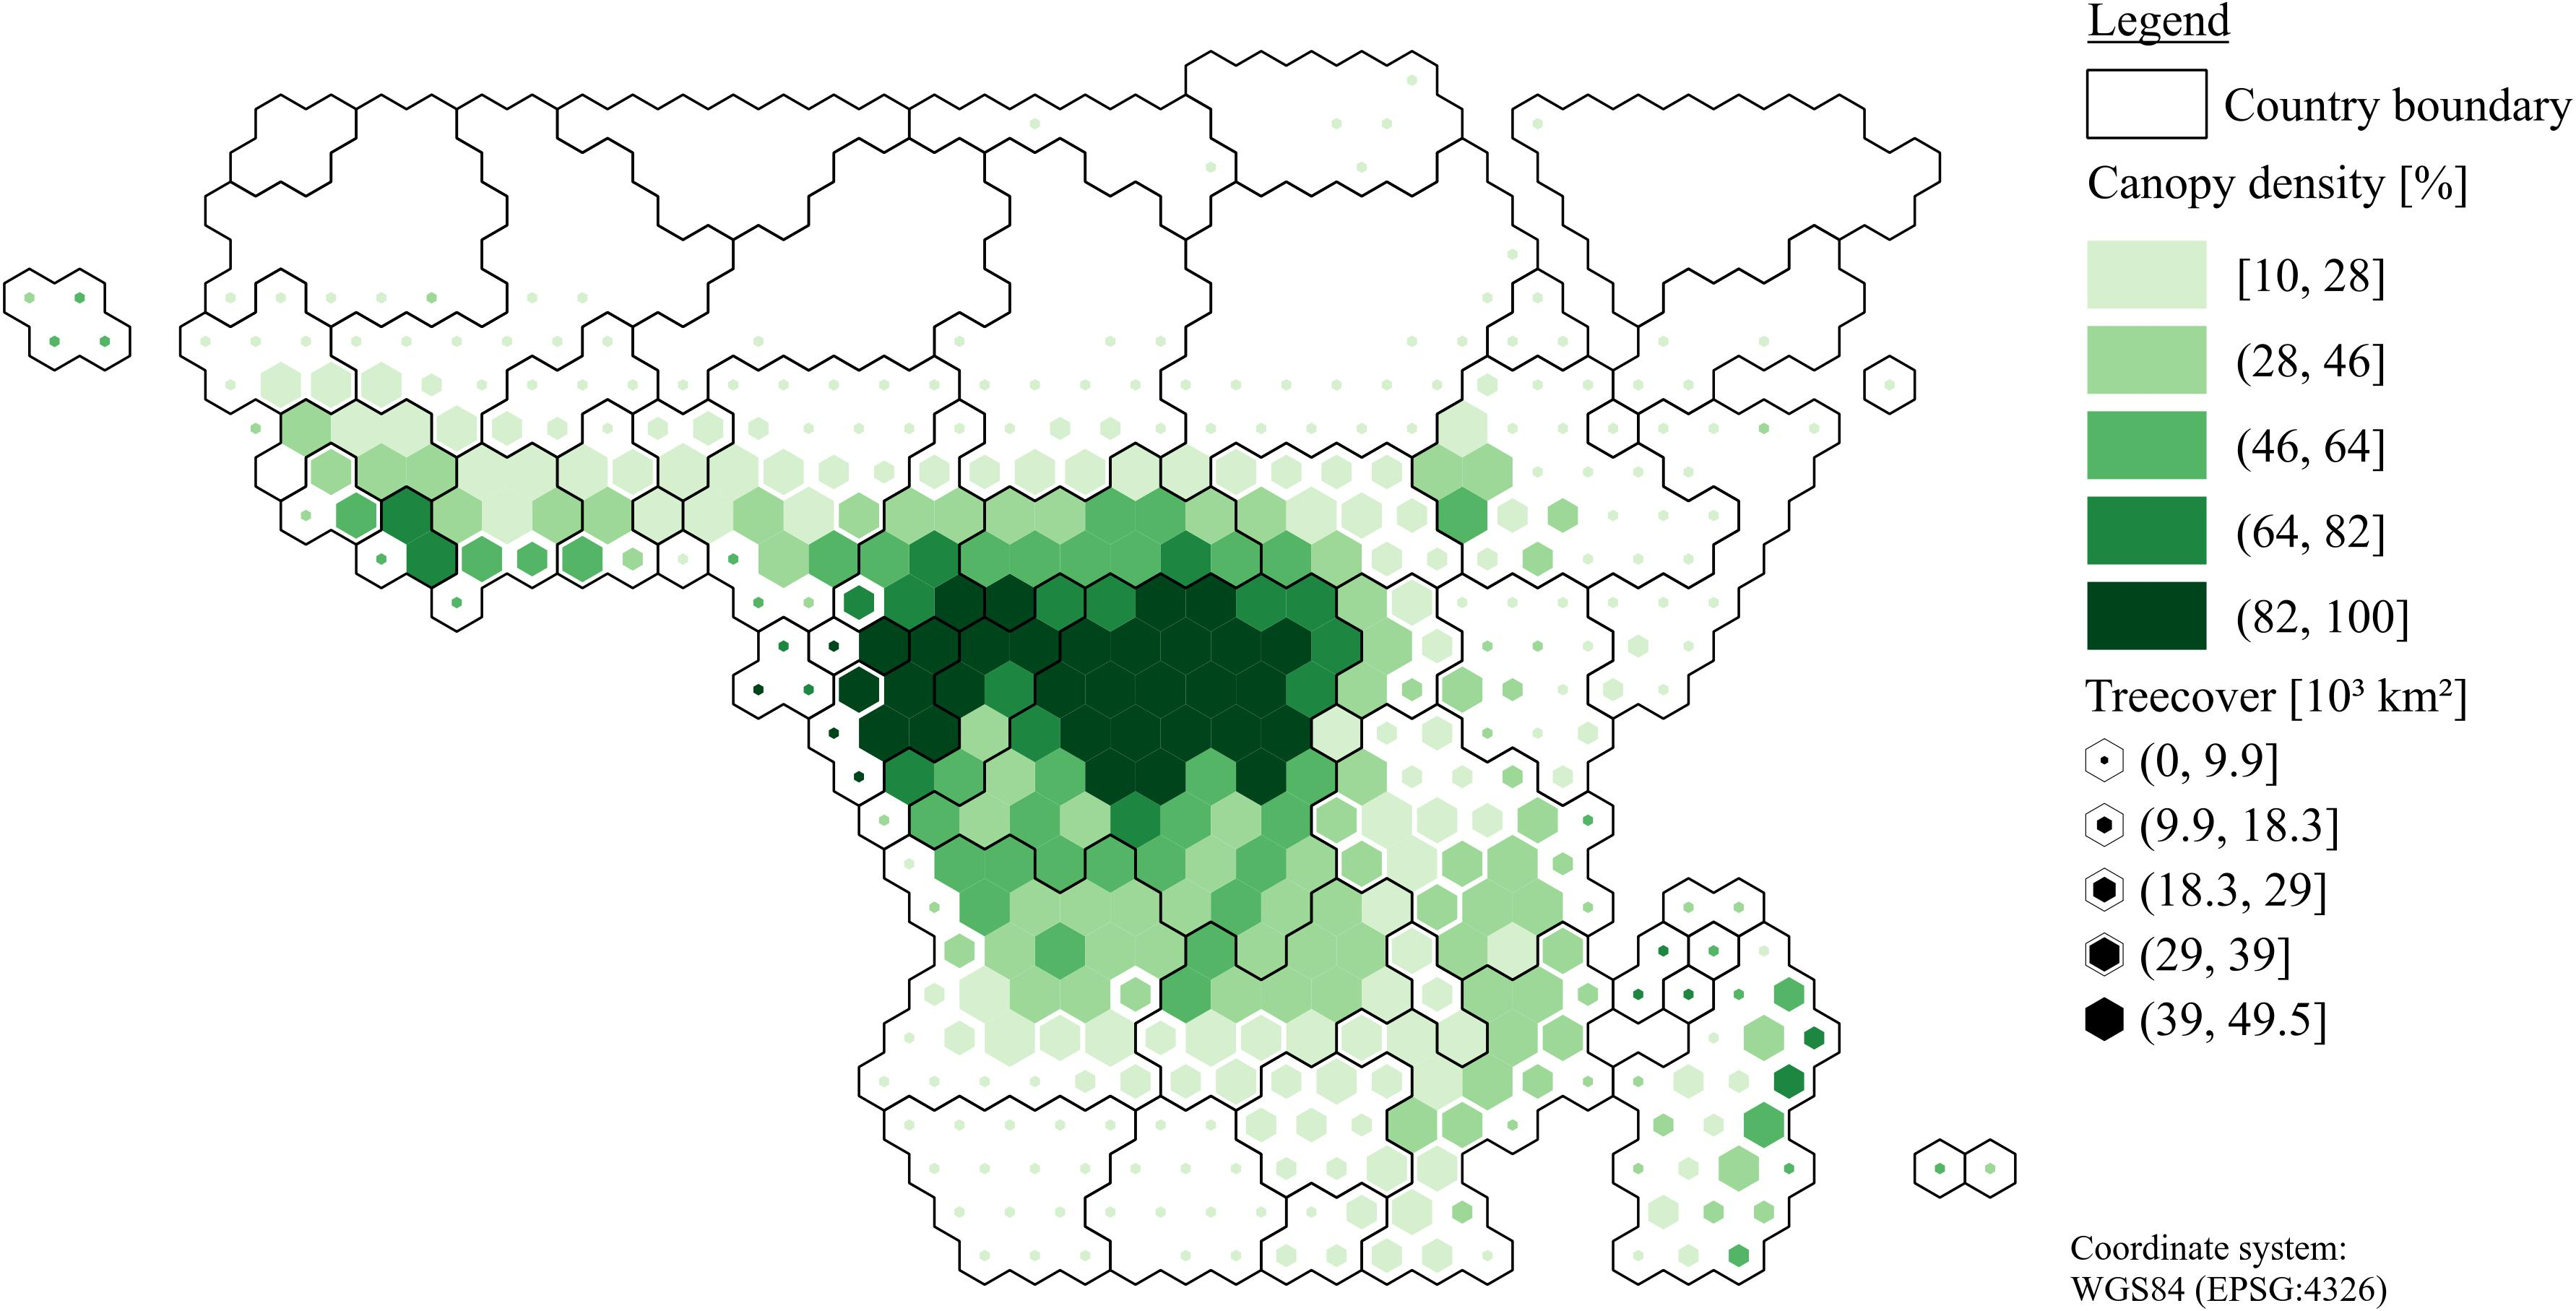
\includegraphics[scale=1]{img/africa_treecover_frameless}
				\caption[Ecosystem service values]{}
				\label{fig:africacover}
			\end{figure}
			\begin{figure}[ht]
				\centering
				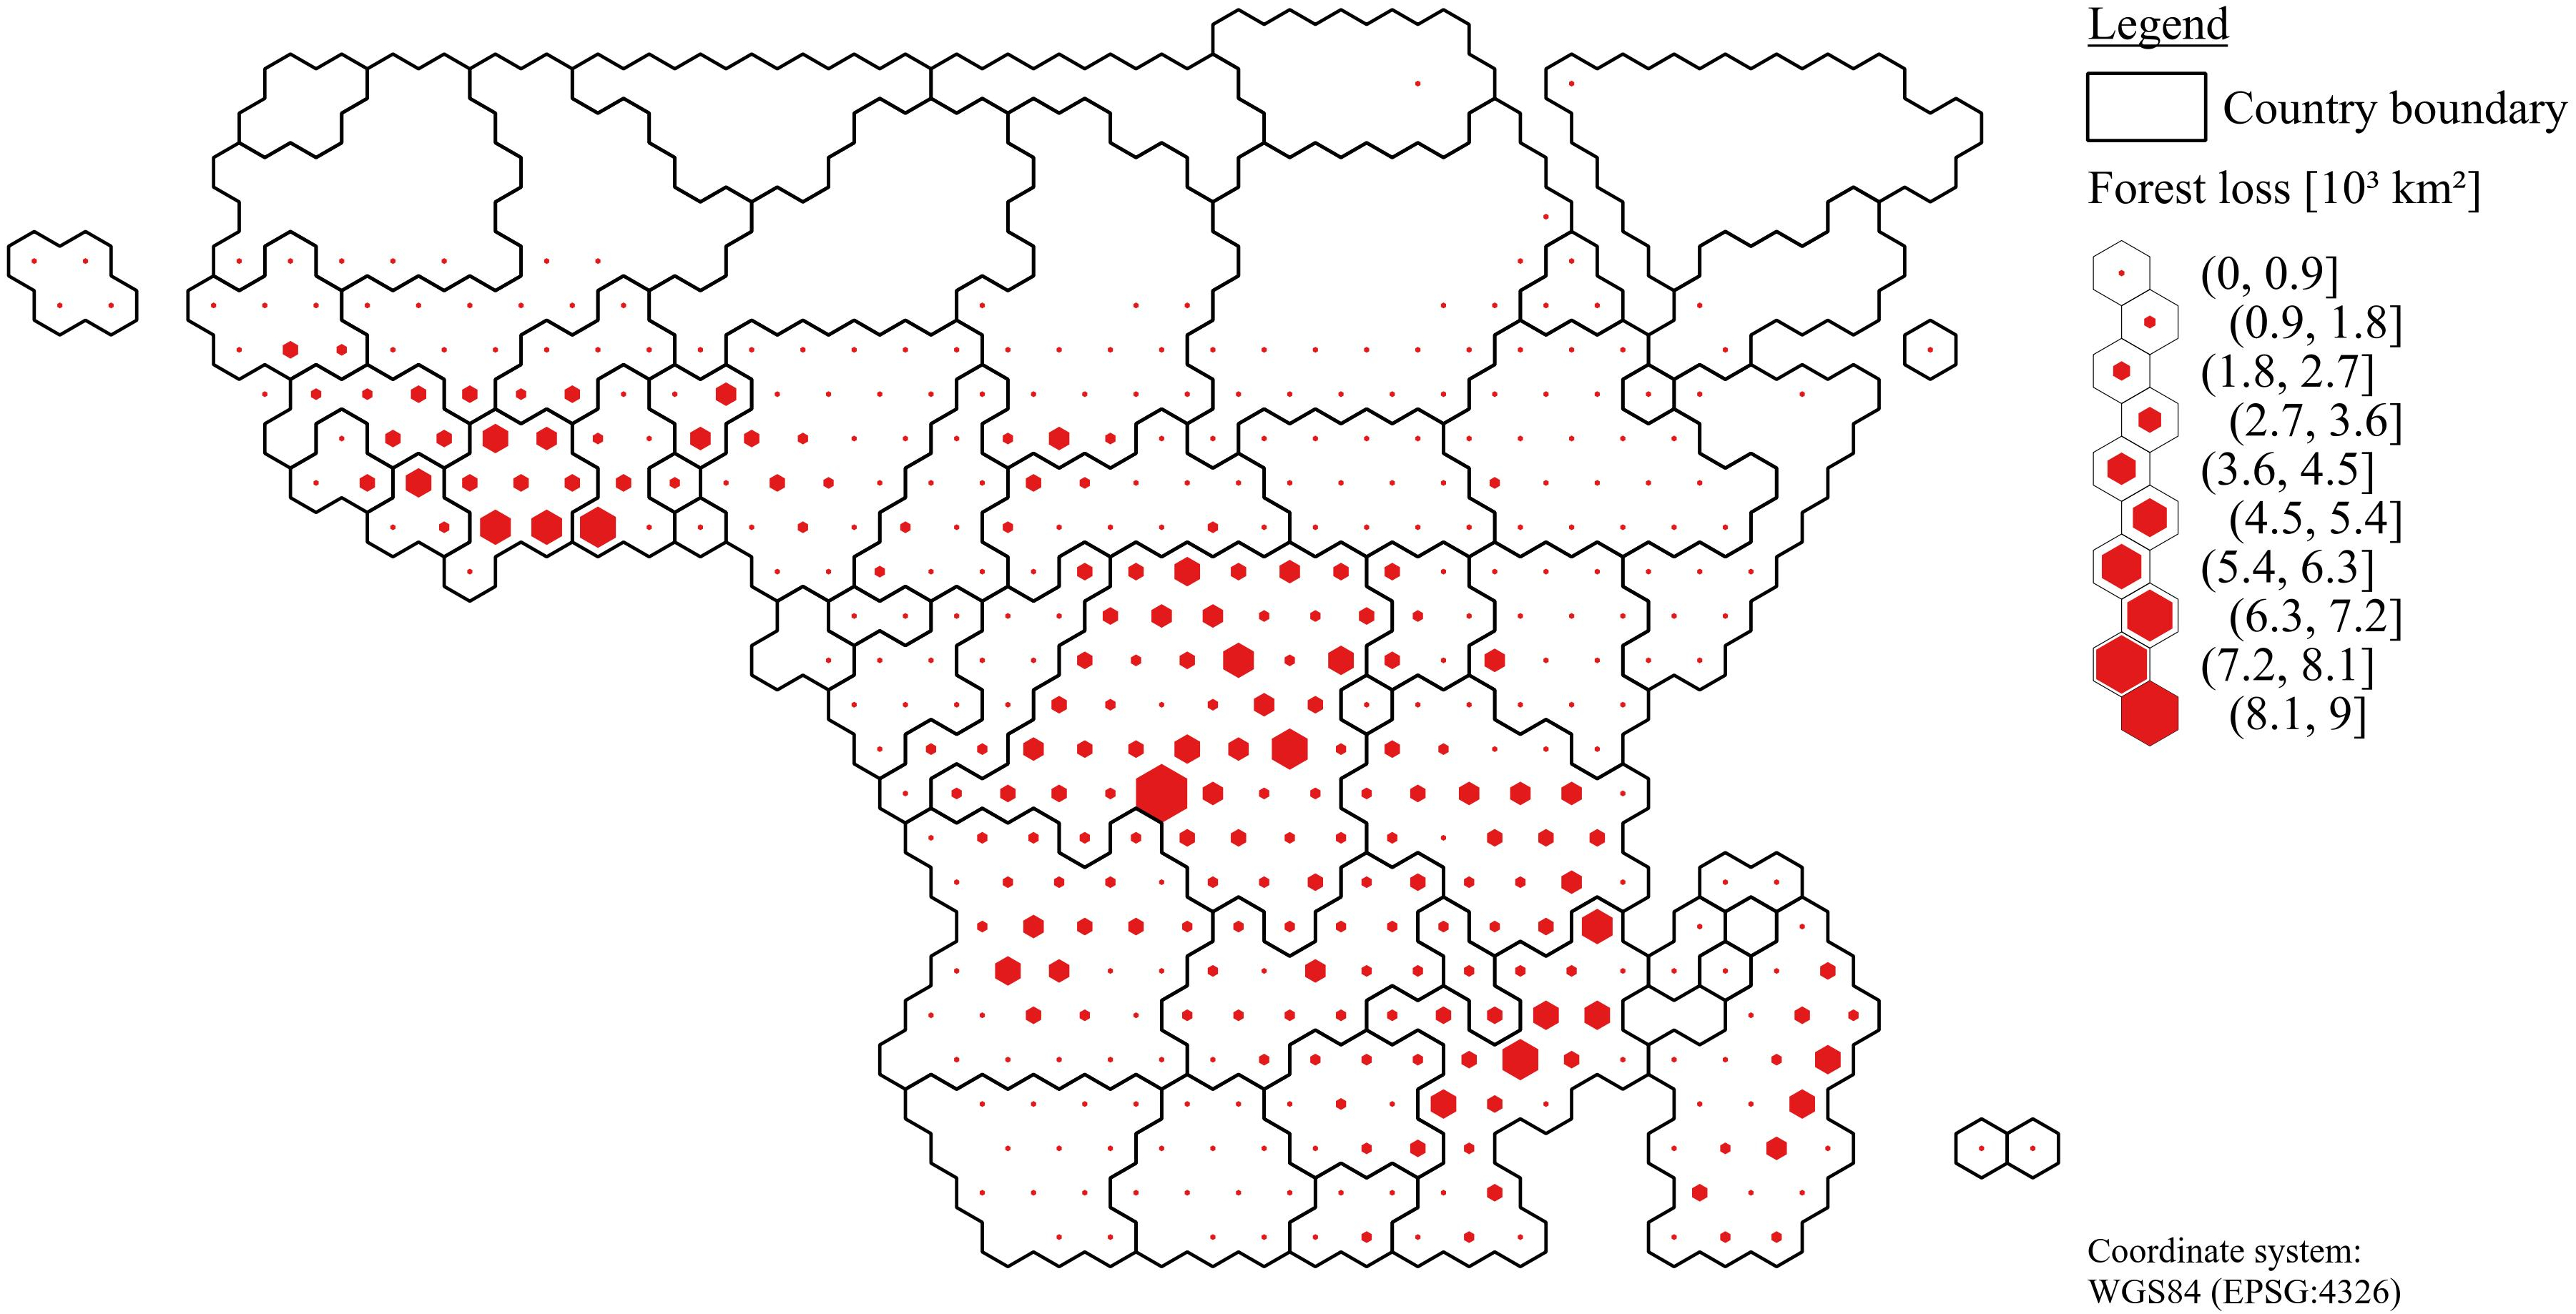
\includegraphics[scale=1]{img/africa_loss_frameless}
				\caption[Ecosystem service values]{}
				\label{fig:africaloss}
			\end{figure}
			\begin{figure}[ht]
				\centering
				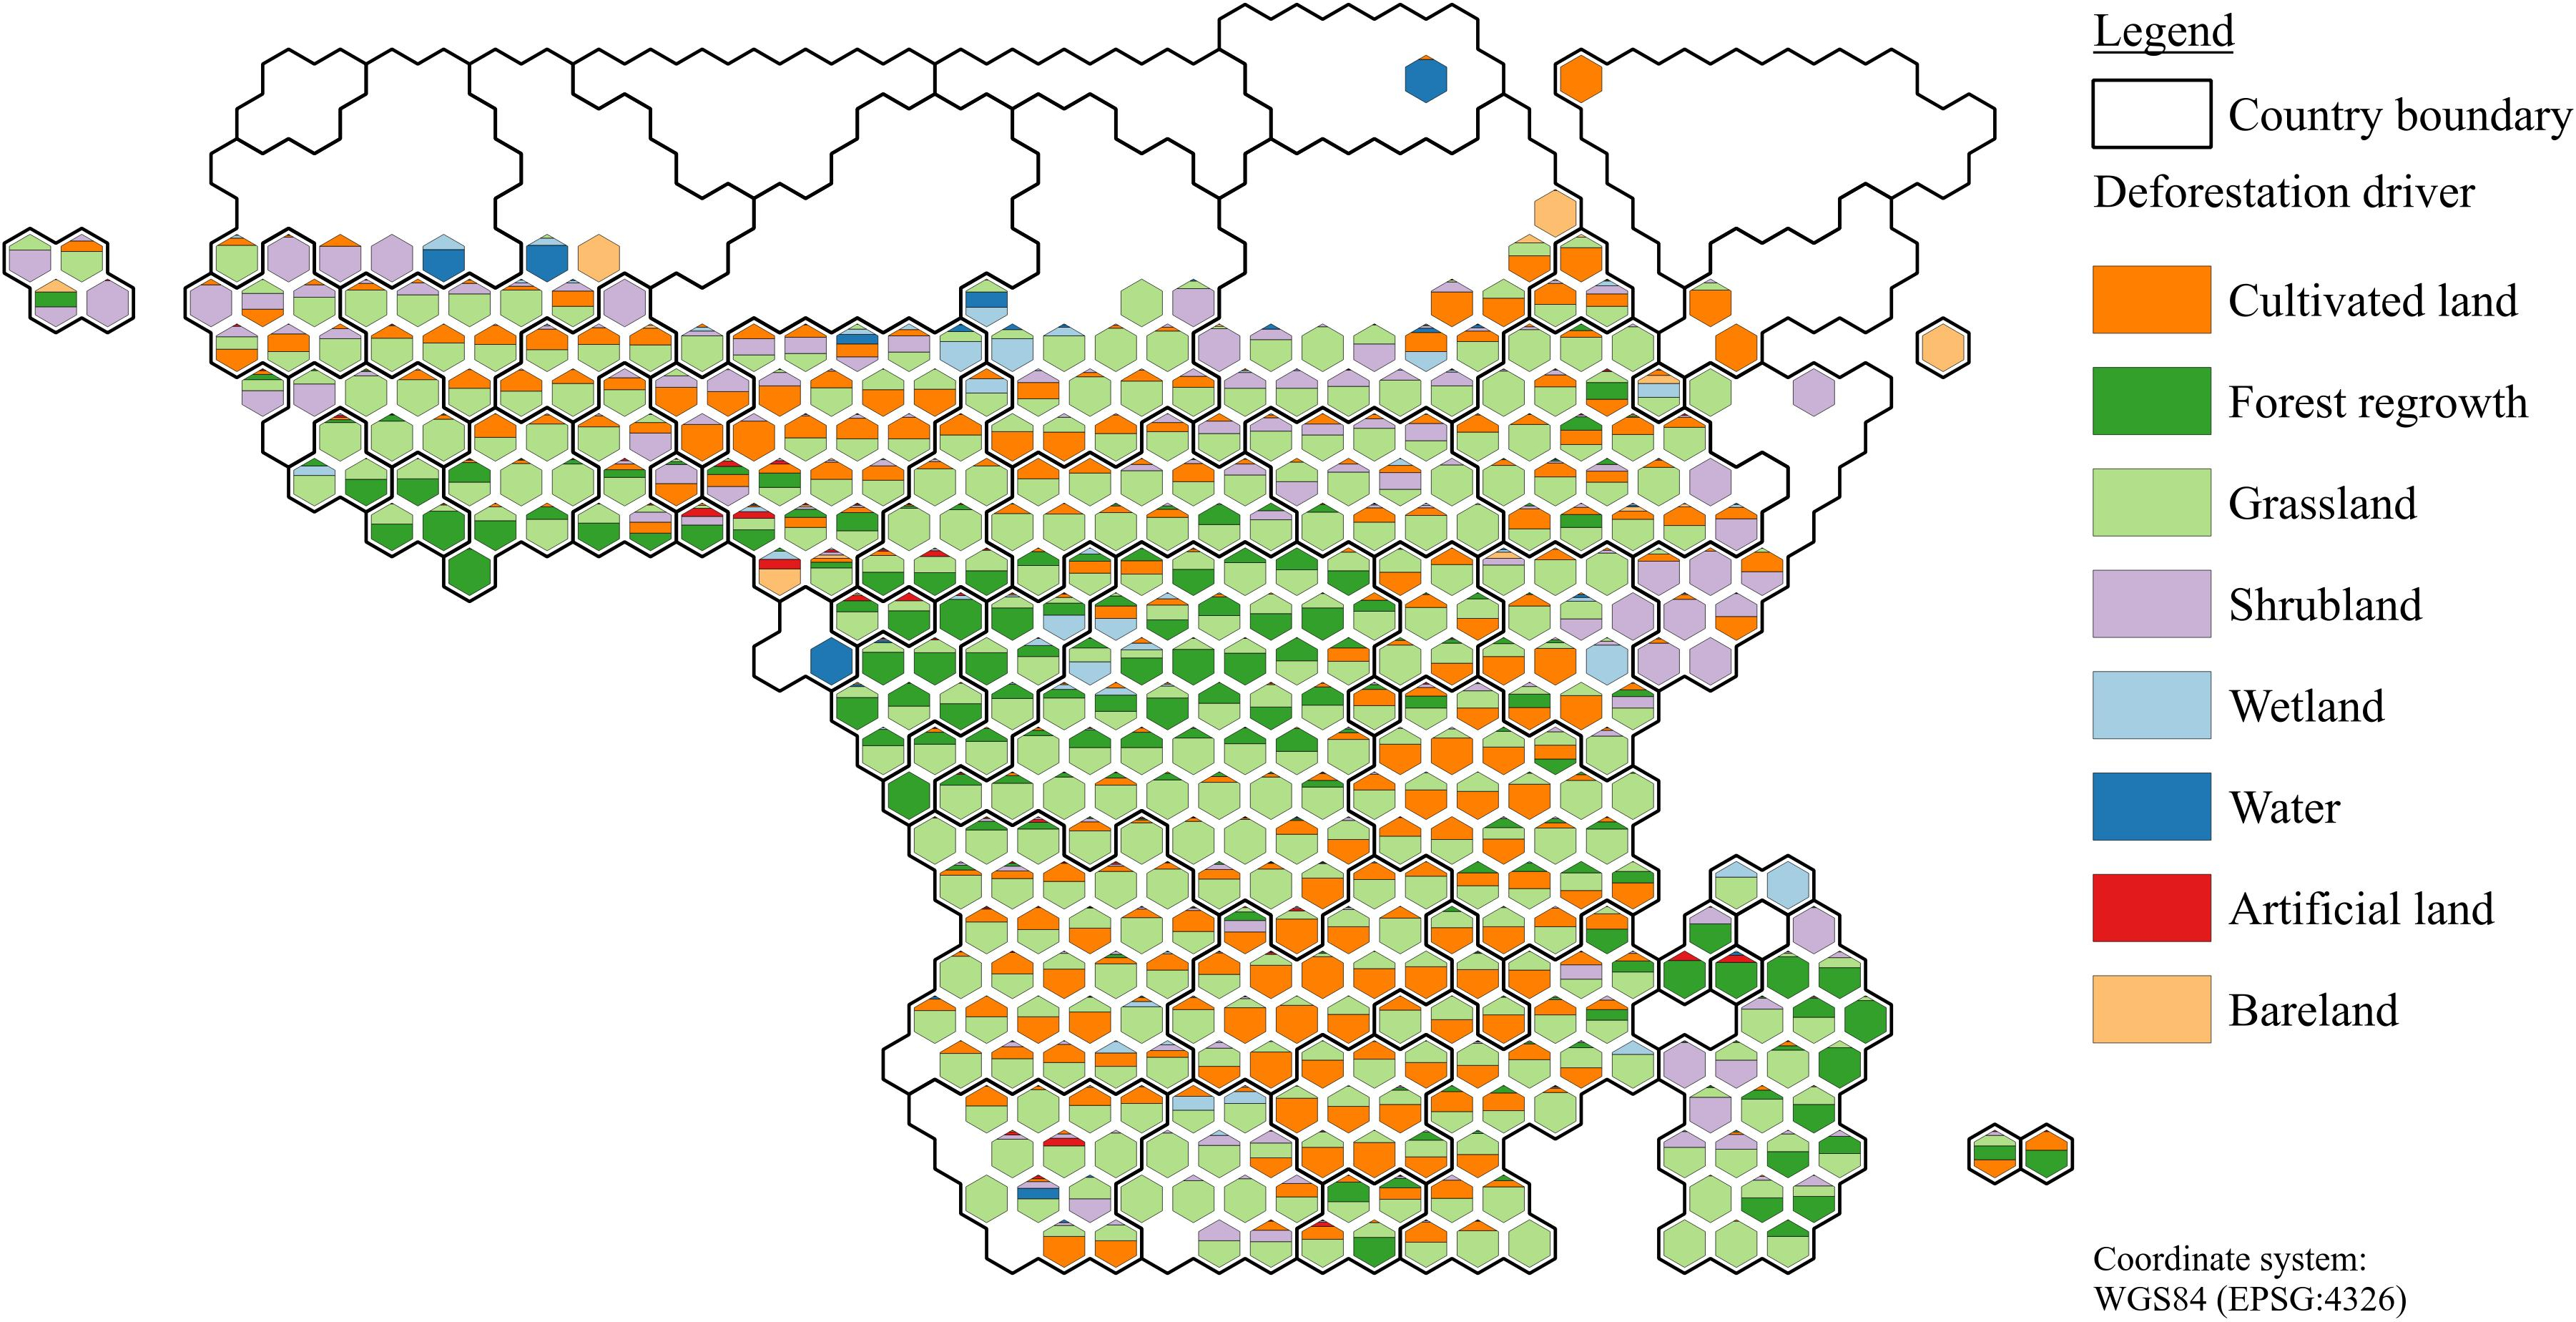
\includegraphics[scale=1]{img/africa_driver_frameless}
				\caption[Ecosystem service values]{}
				\label{fig:africadriver}
			\end{figure}

\clearpage

	\section{Deforestation emissions}
	\label{sec:emissions}
	%TODO landscape img from agb emissions and soc emissions
	%TODO table of soc emissions (global and continental) per driver
	%TODO table of agb emissions (global and continental) per driver
	%TODO graph soc emissions include global
	%TODO graph agb emissions include global

		\begin{figure}[ht]
			\centering
			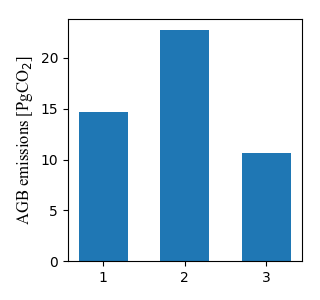
\includegraphics[scale=1]{img/agbe}
			\caption[Ecosystem service values]{}
			\label{fig:agbe}
		\end{figure}
		\begin{figure}[ht]
			\centering
			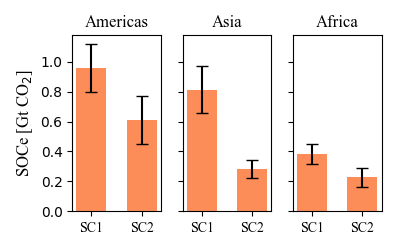
\includegraphics[scale=1]{img/soce}
			\caption[Ecosystem service values]{}
			\label{fig:soce}
		\end{figure}
		
		
		\begin{table}[ht]
			\centering
			\caption[Soil organic carbon emissions]{Soil organic carbon emissions}
			\label{tab:soce_tab}
			\begin{tabular}{lrrrrrrrrr}
				\hline
				\multirow{3}{*}{Region} & \multicolumn{3}{c}{SC1}& \multicolumn{3}{c}{SC2} & \multicolumn{3}{c}{SC3} \\
				& \multicolumn{3}{c}{[Gt CO$_2$]}& \multicolumn{3}{c}{[Gt CO$_2$]} & \multicolumn{3}{c}{[Gt CO$_2$]} \\
				& min & mean & max & min & mean & max & min & mean & max \\\hline
				Americas & 0.80 & 0.96 & 1.12 & 0.45 & 0.61 & 0.77 & 0.43 & 0.59 & 0.76 \\
				Asia & 0.66 & 0.81 & 0.97 & 0.22 & 0.28 & 0.34 & 0.22 & 0.28 & 0.33 \\
				Africa & 0.32 & 0.39 & 0.45 & 0.17 & 0.23 & 0.29 & 0.16 & 0.23 & 0.29 \\\hline
			\end{tabular}
		\end{table}

		\subsection{Global}
		\subsection{Americas}
		\subsection{Asia}
		\subsection{Africa}

	\section{Ecosystem service value balance}
	%TODO table of ecosystem service value losses per driver

		\begin{figure}[ht]
			\centering
			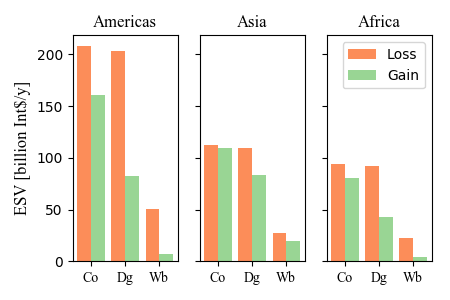
\includegraphics[scale=1]{img/esv}
			\caption[Ecosystem service values]{}
			\label{fig:esv}
		\end{figure}

	\subsection{Global}
	\subsection{Americas}
	\subsection{Asia}
	\subsection{Africa}
